%=============================================================================
% Traffic Digital Twin — IEEE conference report (BASE version, no Contribution)
% Compile: pdflatex report_base ; bibtex report_base ; pdflatex report_base x2
% Or upload the report/ folder to Overleaf and compile report_base.tex.
%=============================================================================
\documentclass[conference]{IEEEtran}
\IEEEoverridecommandlockouts

\usepackage{cite}
\usepackage{amsmath,amssymb,amsfonts}
\usepackage{algorithm}
\usepackage{algpseudocode}
\usepackage{graphicx}
\usepackage{booktabs}
\usepackage{multirow}
\usepackage{textcomp}
\usepackage{xcolor}
\usepackage{tikz}
\usetikzlibrary{shapes.geometric, arrows.meta, positioning, fit, backgrounds}
\usepackage[hidelinks]{hyperref}
\usepackage{url}
\usepackage[final]{microtype}
\usepackage{makecell}

% Long monospaced identifiers (e.g. transform.py:\_pixel\_to\_gps\_curved) cannot
% break in the narrow IEEE columns and cause large inter-word gaps. Allow a break
% after every underscore and relax justification slightly to remove the rivers.
\renewcommand{\_}{\textunderscore\allowbreak}
\setlength{\emergencystretch}{3em}

\graphicspath{{img/}{figures/}{../poster/}{report/img/}}

% Compile-safe figure: include the image if present (searched in figures/ and
% ../poster/ via \graphicspath), else draw a labelled placeholder. \detokenize keeps
% underscores in filenames from being read as math.
\newcommand{\figorbox}[2]{%
  \IfFileExists{img/#1}{\includegraphics[width=\linewidth]{#1}}{%
  \IfFileExists{figures/#1}{\includegraphics[width=\linewidth]{#1}}{%
  \IfFileExists{report/img/#1}{\includegraphics[width=\linewidth]{#1}}{%
  \IfFileExists{../poster/#1}{\includegraphics[width=\linewidth]{#1}}{%
  \IfFileExists{#1}{\includegraphics[width=\linewidth]{#1}}{%
    \fbox{\parbox[c][3.2cm][c]{0.92\linewidth}{\centering\small\itshape
      [figure placeholder: \texttt{\detokenize{#1}}]\\#2}}}}}}}}

\begin{document}

\title{A Real-Time Traffic Digital Twin from Public CCTV:\\
Vision-Based Detection, Map-Anchored Localization, and Self-Calibrating Speed Estimation}

\author{
\IEEEauthorblockN{Minsoo Ahn}
\IEEEauthorblockA{Department of Computer Science\\
Stony Brook University\\
minsoo.ahn@stonybrook.edu}
\and
\IEEEauthorblockN{Dahyun Kwon}
\IEEEauthorblockA{Department of Computer Science\\
Stony Brook University\\
dahyun.kwon@stonybrook.edu}
}

\maketitle

%-----------------------------------------------------------------------------
\begin{abstract}
We present a real-time traffic digital twin that converts live public CCTV feeds
into an interactive, map-anchored view of road traffic. The system detects vehicles
with YOLO26, tracks them with BoxMOT, and projects each pixel position to a
geographic coordinate via a perspective homography. Because public CCTV cameras are
uncalibrated, accurate ground-plane mapping and speed estimation are the central
challenges. We address them with three mechanisms: (i) a two-stage curved transform
that maps pixels along the true road centreline from the national node-link road
network; (ii) a five-stage speed estimator with physics-based outlier rejection,
sliding-window least-squares regression, and per-track exponential smoothing; and
(iii) a per-camera scale factor updated online via an ITS-referenced calibration
loop. The homography itself is produced without manual setup by a warm-up pipeline
that builds a vehicle-free \emph{clean plate} to expose lane markings and solve camera
pose, recovering the focal length geometrically when dashed markings are visible. The
system additionally supports multi-camera background monitoring,
congestion clustering, and a SQLite time-series history. We describe the
architecture and key algorithms, and report latency, throughput, tracking
stability, and localization accuracy over live streams.
\end{abstract}

\begin{IEEEkeywords}
digital twin, intelligent transportation systems, object detection, multi-object
tracking, homography, perspective transform, speed estimation, real-time
visualization.
\end{IEEEkeywords}

%=============================================================================
\section{Introduction}
%=============================================================================
Cities expose thousands of public traffic cameras, but the raw feeds are difficult
to interpret at scale: an operator watching a video grid cannot read off vehicle
counts, speeds, or where congestion is forming on a map. A \emph{digital twin}---a
live, geo-referenced model of the road state---turns those feeds into actionable
information. The technical obstacle is that public CCTV cameras are
\emph{uncalibrated}: their height, pitch, focal length, and exact heading are
unknown, so projecting an image detection onto the ground plane (and therefore
measuring distance and speed) is ill-posed without per-camera calibration.

This paper describes a system that ingests Korean ITS CCTV streams and produces a
real-time map-anchored twin. Our contributions, from a systems and algorithms
standpoint, are:

\begin{itemize}
  \item \textbf{Map-anchored localization.} We snap each camera onto the national
  node-link road network, extract the road centreline, and map pixels along the
  \emph{curve} of the road in two stages, rather than assuming a flat homographic
  plane. Satellite-referenced landmarks (Section~\ref{sec:eval}) show the pipeline
  places vehicles with $1.8$--$10.3$\,m lateral (on-road) accuracy; the curved stage
  constrains markers to the mapped road shape on bends without degrading an
  already-accurate flat fit.
  \item \textbf{Robust speed estimation without ground truth.} A five-stage filter
  (duplicate skip, physics jump guard, sliding-window least-squares regression,
  per-track exponential smoothing with spike rejection, and scale correction)
  produces stable speeds despite detection jitter and tracker ID churn.
  \item \textbf{Per-camera scale correction.} Because absolute distance scale is
  unknowable from an uncalibrated camera whenever the geometric focal-free solve cannot
  fire, the system maintains a per-camera \texttt{speed\_scale} that absorbs the residual
  longitudinal scale error and decouples geometric projection from absolute speed
  accuracy. An ITS-referenced online update loop with adaptive rate $\alpha_s$ (0.15 initially, decaying to 0.01) accumulates the factor across sessions; the current deployment has collected
  factors for 48 cameras (range 0.34--2.25), though multi-session operation is required for full convergence (see Section~\ref{sec:discuss}).
  \item \textbf{A complete, resilient pipeline.} A warm-up clean-plate auto-calibration
  that solves camera pose with focal-free longitudinal anchoring and locks once committed
  (manual 4-point calibration available), dual-path inference (browser canvas and
  server-side HLS) over a shared detector, multi-camera background monitoring, congestion
  clustering, and a historical analytics store.
\end{itemize}

The rest of the paper is organized as follows. Section~\ref{sec:related} reviews
related work and positions this system relative to the state of the art.
Section~\ref{sec:design} presents the system architecture.
Section~\ref{sec:impl} details the algorithms. Section~\ref{sec:eval} reports the
measurements. Section~\ref{sec:discuss} discusses limitations, and
Section~\ref{sec:concl} concludes.

%=============================================================================
\section{Related Work}\label{sec:related}
%=============================================================================
\textbf{Object detection and tracking.} Modern traffic vision builds on real-time
detectors. NMS-based architectures such as YOLOv8~\cite{yolov8} suppress redundant
boxes through non-maximum suppression, but the threshold-sensitivity of NMS causes
bounding-box positions to jitter between frames; this per-frame noise propagates
directly into downstream speed estimates. To eliminate the source of positional
instability, we adopt YOLO26~\cite{yolo26}, an NMS-free end-to-end detector that
produces more consistent bounding-box positions and simplifies the TensorRT FP16
engine graph by removing the NMS layer~\cite{tensorrt}, lowering both inference
latency and its variance; YOLOv8 is retained as a legacy fallback. For tracking we use the BoxMOT
framework~\cite{boxmot}, which exposes ByteTrack~\cite{bytetrack},
BoT-SORT~\cite{botsort}, and OC-SORT~\cite{ocsort}; appearance re-identification
uses OSNet~\cite{osnet}. Trackers without appearance ReID suffer ID switches under
occlusion, which we mitigate with a lightweight position-based ID stabilizer.

\textbf{Camera-to-ground mapping.} Mapping image points to a ground plane is a
homography problem~\cite{hartley2004}, typically solved from four correspondences
with OpenCV~\cite{opencv}. For \emph{uncalibrated} cameras, vanishing-point and
lane-geometry cues are commonly used to recover pose~\cite{dubska2014}, but these techniques assume
the ground plane is locally flat---an assumption that introduces lateral
displacement errors of several metres on curved roads.
Dubska et al.~\cite{dubska2014} achieve fully automatic calibration of roadside
cameras from lane markings and vanishing points, but their model is restricted to
a flat road plane; our pose solver extends this by additionally recovering camera
height and pitch, and a second curved-centreline stage corrects residual lateral
displacement on bends. To follow actual road
geometry, our work introduces a road-centreline-following transform driven by a
national road-network dataset~\cite{moct_nodelink}, alongside a 4-point manual
mode and a vanishing-point/lane auto-calibration path.

\textbf{ITS dashboards and data.} National ITS portals~\cite{its_openapi} publish
CCTV streams and aggregated segment speeds, but typically as separate views; the
aggregated speed is never fed back to correct the vision-derived estimate, leaving
any geometric scale error unchecked. We bridge this gap by \emph{fusing} the
segment speed into the pipeline as an online calibration signal for per-camera
scale correction.
Congestion grouping uses density-based clustering~\cite{dbscan} and convex
hulls~\cite{andrew1979}; service levels follow the Highway Capacity
Manual~\cite{los_hcm}. The visualization uses deck.gl~\cite{deckgl} over
MapLibre~\cite{maplibre}, served by FastAPI~\cite{fastapi}.


\subsection{Positioning Relative to State of the Art}\label{sec:sota}
We position this work against representative monocular traffic-analysis systems
along the dimensions most relevant to uncalibrated public-infrastructure
deployment. Table~\ref{tab:sota} summarises the comparison; the discussion below
groups the prior art into three families and states explicitly where our system
agrees with, differs from, and is limited relative to each.

\begin{table*}[t]
\caption{Comparison with representative traffic-monitoring approaches.
\checkmark~=~fully supported; $\times$~=~not supported; $\triangle$~=~partially supported; ---~=~not applicable.}
\label{tab:sota}
\centering
\scriptsize
\begin{tabular}{@{}lcccccccc@{}}
\toprule
\textbf{Method} &
\makecell{\textbf{No road}\\\textbf{HW}} &
\makecell{\textbf{No vehicle}\\\textbf{GPS}} &
\makecell{\textbf{Auto-}\\\textbf{calib}} &
\makecell{\textbf{Curved}\\\textbf{road}} &
\makecell{\textbf{Speed}\\\textbf{est.}} &
\makecell{\textbf{Real-}\\\textbf{time}} &
\makecell{\textbf{Multi-}\\\textbf{cam}} &
\makecell{\textbf{Open-}\\\textbf{source}} \\
\midrule
Loop / Radar sensors       & $\times$ & \checkmark & ---        & ---        & \checkmark & \checkmark & $\triangle$ & $\times$   \\
On-vehicle GPS             & \checkmark & $\times$ & ---        & \checkmark & \checkmark & \checkmark & \checkmark  & $\triangle$ \\
YOLO + flat homography     & \checkmark & \checkmark & $\times$ & $\times$   & $\triangle$ & \checkmark & $\times$   & \checkmark \\
Dubsk\'a et al.~\cite{dubska2014} & \checkmark & \checkmark & \checkmark & $\times$ & \checkmark & \checkmark & $\times$ & $\times$ \\
Sochor et al.~\cite{sochor2019} & \checkmark & \checkmark & \checkmark & $\times$ & \checkmark & \checkmark & $\times$ & \checkmark \\
Revaud \& Humenberger~\cite{revaud2021} & \checkmark & \checkmark & \checkmark & $\triangle$ & \checkmark & \checkmark & $\times$ & \checkmark \\
\textbf{This work}         & \checkmark & \checkmark & \checkmark & \checkmark & \checkmark & \checkmark & \checkmark & \checkmark \\
\bottomrule
\end{tabular}
\end{table*}


\textbf{Closest setting: monocular CCTV speed estimation.}
The most directly comparable line of work estimates vehicle speed from a single
uncalibrated surveillance camera. Sochor et al.~\cite{sochor2019} established the
de-facto benchmark for this task, BrnoCompSpeed, with LIDAR-derived ground-truth
speeds, and report sub-km/h mean error on full-HD footage of predominantly
straight motorway segments. Revaud and Humenberger~\cite{revaud2021} target the
same problem under realistic CCTV conditions---explicitly including low-resolution
and non-straight roads---and, notably, evaluate on a dataset of Korean public CCTV
streams with GPS-traced ground truth, the same infrastructure family this work
builds on. Their calibration leverages the known 3D dimensions of vehicles;
ours instead leverages the known 2D geometry of the road from the national
node-link network. The two priors are complementary: a 3D-vehicle prior recovers
metric scale per detection, whereas our centreline prior recovers road-following
position over an extended corridor. We note that although the Revaud data
\emph{includes} non-straight roads, their method estimates speed without anchoring
each vehicle to the road's mapped curvature; it is robust \emph{on} curved scenes
but does not constrain positions \emph{to} the curve, which is why we mark it
partial ($\triangle$) rather than full in the ``Curved road'' column of
Table~\ref{tab:sota}. FARSEC~\cite{farsec2023} subsequently provided
a reproducible pipeline evaluated on both BrnoCompSpeed and the Revaud CCTV set,
underscoring that these two datasets are the accepted reference points for the
task.

We emphasise an honest distinction. These methods report quantitative speed
accuracy against instrumented ground truth, which our present evaluation does not:
our speed figures (Table~\ref{tab:track}) confirm plausible output rather than
benchmark accuracy, and the per-camera \texttt{speed\_scale} factors remain
unconverged at the time of writing. We do, however, validate \emph{localization}
quantitatively against satellite-referenced landmarks (Section~\ref{sec:eval}),
which is the dimension we claim as the contribution. Establishing comparable speed
accuracy on the Revaud Korean-CCTV set or BrnoCompSpeed is the natural next step and
is left as future work; the contribution claimed here is the map-anchored
localization and self-calibrating pipeline, not a new speed-accuracy record.

\textbf{Automatic calibration from road geometry.}
A second family recovers camera pose automatically from lane markings and
vanishing points. Dubsk\'a et al.~\cite{dubska2014} achieve fully automatic
calibration of roadside cameras from these cues, and Sochor et
al.~\cite{sochor2019} refine scene scale by aligning 3D vehicle bounding boxes,
reducing scale error substantially over earlier automatic methods. Both, however,
model the road as a single flat plane. Our pose solver
(\texttt{camera\_pose.solve\_pose}) follows the same vanishing-point/lane-edge
strategy but additionally recovers camera height and pitch against a known road
width, and---critically---a second centreline-following stage
(Algorithm~\ref{alg:curved}) corrects the residual lateral displacement that a
flat-plane model leaves on bends. This is the dimension labelled ``Curved road''
in Table~\ref{tab:sota}, where prior monocular methods are marked unsupported.

\textbf{Dedicated sensors and on-vehicle GPS.}
A third family sidesteps calibration entirely. Inductive-loop detectors, roadside
radar, and on-vehicle GPS loggers measure speed and position directly, but require
either physical roadside installation or instrumentation of the vehicles
themselves. Our system adds no hardware to the road or to vehicles, re-purposing
cameras that road authorities already operate; the trade-off is that all geometry
is inferred and therefore bounded by the quality of the map and the perspective
projection (Section~\ref{sec:discuss}).

\textbf{Generic detection/tracking pipelines.}
Finally, open-source YOLO+BoxMOT pipelines provide bounding boxes and track IDs but
no geographic anchoring, calibrated speed, or support for uncalibrated cameras out
of the box. Our system integrates these components and adds the localization,
calibration, and self-correction layers that turn raw tracks into a map-anchored
twin. Among the compared systems, ours is the only one supporting the full set of
columns in Table~\ref{tab:sota}; we nonetheless note that this breadth reflects a
systems-integration contribution rather than a single-metric advance, and that the
per-axis novelty (curved localization, ITS-referenced scale) is what we claim as
new.

%=============================================================================
\section{System Design and Architecture}\label{sec:design}
%=============================================================================
The backend (FastAPI/Uvicorn) and a React/deck.gl frontend communicate over REST
and WebSocket. Two inference paths can produce per-frame analytics and
\emph{share a single detector}; a connection counter coordinates them so that the
multi-object tracker is never driven by two interleaved frame streams
(Fig.~\ref{fig:arch}). A two-lock scheme inside the detector
(\texttt{\_state\_lock} for tracker state, \texttt{\_lock} for GPU inference)
prevents data races between thread-pool threads, and module-level write locks
in \texttt{main.py} and \texttt{roi\_manager.py} atomize all JSON configuration
read-modify-write operations.

\begin{figure*}[t]
\centering
% --- Architecture diagram (TikZ; two-column wide, self-contained) ---
\resizebox{0.95\linewidth}{!}{%
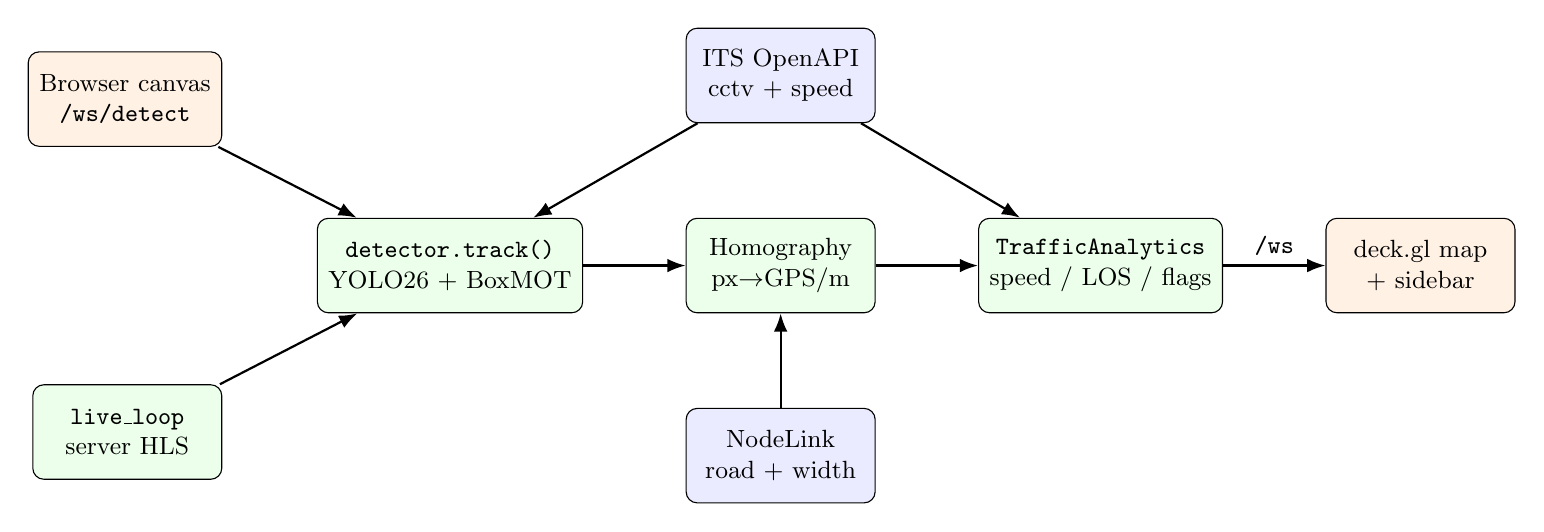
\begin{tikzpicture}[
  box/.style={draw, rounded corners, align=center, font=\small, inner sep=4pt,
              minimum height=12mm, minimum width=24mm},
  ext/.style={box, fill=blue!8},
  be/.style={box, fill=green!8},
  fe/.style={box, fill=orange!10},
  arr/.style={-{Latex}, thick}]

  % main pipeline (single row, left to right)
  \node[be] (det) {\texttt{detector.track()}\\YOLO26 + BoxMOT};
  \node[be, right=13mm of det] (tf) {Homography\\px$\to$GPS/m};
  \node[be, right=13mm of tf] (an) {\texttt{TrafficAnalytics}\\speed / LOS / flags};
  \node[fe, right=13mm of an] (ws) {deck.gl map\\+ sidebar};

  % two inputs merge into the shared detector (left side)
  \node[fe, above left=9mm and 12mm of det] (canv) {Browser canvas\\\texttt{/ws/detect}};
  \node[be, below left=9mm and 12mm of det] (live) {\texttt{live\_loop}\\server HLS};

  % external data sources (above / below the centre, short non-crossing arrows)
  \node[ext, above=12mm of tf] (its) {ITS OpenAPI\\cctv + speed};
  \node[ext, below=12mm of tf] (nl)  {NodeLink\\road + width};

  \draw[arr] (canv) -- (det);
  \draw[arr] (live) -- (det);
  \draw[arr] (det)  -- (tf);
  \draw[arr] (tf)   -- (an);
  \draw[arr] (an)   -- node[above,font=\small]{\texttt{/ws}} (ws);
  \draw[arr] (nl)   -- (tf);
  \draw[arr] (its)  -- (det);
  \draw[arr] (its)  -- (an);
\end{tikzpicture}}
\caption{System architecture. The browser path (\texttt{/ws/detect}) and the
server path (\texttt{live\_loop}) share one detector; a counter prevents concurrent
tracker calls. External data (ITS CCTV/speed, NodeLink) feeds localization and
self-calibration.}
\label{fig:arch}
\end{figure*}

Because running a separate detector per connection would multiply GPU memory use
and violate the shared-tracker invariant, both paths feed a single shared detector;
the connection counter ensures only one path drives the multi-object tracker at a
time. The two paths are designed for complementary operating conditions.

\textbf{Browser path (\texttt{/ws/detect}).} When an operator opens a camera view,
the frontend plays the HLS stream through a CORS proxy, captures canvas frames
(JPEG, $\le$640\,px, $\approx$33\,ms interval, at most two in flight), and sends
them to the backend, which runs detection, tracking, localization, and analytics,
then returns an annotated frame and broadcasts the analytics JSON to all clients.

\textbf{Server path (\texttt{live\_loop}).} Without an active browser client, the
backend reads HLS directly with OpenCV/FFmpeg and runs the same pipeline. It is
gated twice: it skips tracking while a browser detection client is active (to
protect the shared tracker), and it skips all GPU work when no one is watching (the
frontend reports tab visibility). Before opening any HLS URL the detector
pre-resolves HTTP\,302 redirects (\texttt{\_resolve\_hls\_url}), so FFmpeg
receives a direct endpoint and does not silently fail on delivery-layer redirect
chains.

Beyond the two inference paths, sustained operation requires housekeeping that
neither path handles directly: HLS access tokens expire on a 30-minute cycle, the
ITS speed reference drifts unless polled, and the congestion map must be
periodically refreshed. \textbf{Background services.} Periodic loops therefore
refresh expiring HLS tokens (30\,min), poll the ITS segment speed for
self-calibration (5\,min), and snapshot all monitored cameras into a SQLite history
while recomputing congestion clusters (30\,s). To prevent the FOV polygon from
flickering during auto-calibration, a slow EMA filter stabilizes near/far distance
and road-width estimates, holding the initial accepted value fixed until sufficient
samples accumulate. During the warm-up calibration phase the backend broadcasts a
\texttt{calibrating} message (with elapsed time) every 30 frames so the frontend can show
a progress badge, and emits an \texttt{auto\_calibrated} message carrying the recovered
focal length and the reprojection residual once the pose commits. ROI edits trigger an immediate GPS ring recomputation and
broadcast to keep the map view synchronized. The resulting map view is shown in
Fig.~\ref{fig:map}.

\begin{figure}[t]
\centering
\figorbox{cctv_map.png}{Map view with status-coloured CCTV icons and FOV polygon}
\caption{Map view: public CCTV cameras as status-coloured icons on the vector map;
the selected camera shows its field-of-view polygon and the located vehicles.}
\label{fig:map}
\end{figure}

%=============================================================================
\section{Implementation}\label{sec:impl}
%=============================================================================

\subsection{Detection and Tracking}
The detector loads the fastest available backend---TensorRT FP16 engine, then ONNX
Runtime, then PyTorch---and exports \texttt{.pt}$\to$\texttt{.engine} on first run
when a GPU is present. A tracker \emph{tier} is chosen by GPU memory: ByteTrack
(CPU-only, no CUDA), OC-SORT (low VRAM $\ge$3.5\,GB, occlusion-robust, no ReID),
or BoT-SORT/DeepOC-SORT with OSNet appearance ReID on larger GPUs
($\ge$6\,GB and $\ge$10\,GB respectively). Without appearance ReID, two failure modes degrade practical tracking quality:
detectors occasionally fire more than once on the same vehicle, inflating vehicle
counts, and track identities reset after brief occlusions rather than recovering
the original ID, causing discontinuous trails on the map. To suppress both effects,
the non-ReID tiers include two lightweight robustness layers.
\texttt{\_dedup\_tracks} merges duplicate boxes (IoU\,$>$\,0.3 or centre
distance\,$<$\,40\,px, keeping the older ID), while an \texttt{IDStabilizer}
re-binds a vehicle's previous ID after a brief miss using nearest-centre matching
($\le$80\,px) with a two-pass scheme and stale-mapping purge so display IDs stay
stable and compact. Fig.~\ref{fig:yolo} shows the detection and tracking overlay.

\begin{figure}[t]
\centering
\figorbox{yolo_detect.png}{YOLO detection and multi-object tracking overlay}
\caption{Detection and tracking on a live CCTV frame: bounding boxes, vehicle class,
and stabilized track IDs.}
\label{fig:yolo}
\end{figure}

\subsection{Map-Anchored Localization}
On camera switch we query the national node-link network: we snap the camera
position perpendicularly onto the nearest road polyline, extract $\pm$150\,m of
centreline, and---because each direction is stored as a separate one-way link---we
locate the reverse carriageway and average the two snaps (when 2--40\,m apart) to
recover the true road centre. The chosen road's speed limit, lane count, and width
(\,lanes\,$\times$\,2\,$\times$\,lane-width\,) are derived from NodeLink and attached to the camera.

A single flat homography maps pixels to a plane tangent to the camera's snap
point; on curved roads, this plane diverges from the true centreline and displaces
vehicle markers laterally by several metres. To follow the actual road geometry, we
instead introduce the \emph{two-stage curved transform}
(Algorithm~\ref{alg:curved}). The metric homography $H_m$ is derived from the same
four image--GPS correspondences as the GPS homography, but maps pixel coordinates
to local ENU metres rather than geographic coordinates, providing a metric workspace
in which arc-length displacement can be computed accurately. Stage one maps the
pixel to local metres via $H_m$ and converts the result to a geographic coordinate
via the snap-point anchor (\textsc{EnuToGps}); stage two projects that coordinate
perpendicularly onto the centreline polyline (\textsc{PerpProject},
Algorithm~\ref{alg:perp}), obtaining the true arc length and a signed lateral
offset directly from the nearest point on the curve, then re-applies the lateral
offset perpendicular to the local road bearing at that arc.
This replaces the earlier fixed-bearing decomposition
($d_\parallel = dx\sin b + dy\cos b$), which under-measured the true arc length on
bends and folded the road's own curvature into the lateral term as a spurious
offset; the perpendicular projection follows the bend and eliminates that artifact.

\begin{algorithm}
\caption{Two-stage curved pixel$\rightarrow$GPS transform (perpendicular-projection)}
\label{alg:curved}
\begin{algorithmic}[1]
\Require pixel $(u,v)$; metric homography $H_m$; snap point $p_m$ (ENU m);
         snap GPS $(\phi_0,\lambda_0)$; centreline polyline $C=\{(\phi_i,\lambda_i)\}$
         with cumulative arc lengths $\{\ell_i\}$
\State $(x_m,y_m) \gets H_m \cdot (u,v)$ \Comment{pixel $\rightarrow$ ENU metres}
\State $(dx,dy) \gets (x_m,y_m) - p_m$ \Comment{ENU offset from snap}
\State $(\phi_e,\lambda_e) \gets \textsc{EnuToGps}(\phi_0,\lambda_0,dx,dy)$
\State $(\textit{arc},\, d_\perp) \gets \textsc{PerpProject}\big((\phi_e,\lambda_e),\, C\big)$
       \Comment{nearest point on centreline}
\State $(\phi_c,\lambda_c) \gets \textsc{InterpCenterline}(\textit{arc})$
\State $b_\ell \gets \textsc{RoadBearingAt}(\textit{arc})$
\State \textbf{apply} $d_\perp$ perpendicular to $b_\ell$ at $(\phi_c,\lambda_c)$
\State \Return $(\phi,\lambda)$
\end{algorithmic}
\end{algorithm}

\begin{algorithm}
\caption{\textsc{PerpProject}: perpendicular projection onto centreline}
\label{alg:perp}
\begin{algorithmic}[1]
\Require query point $q=(\phi,\lambda)$; centreline $C=\{(\phi_i,\lambda_i)\}$
         with arc lengths $\{\ell_i\}$
\State $d^\star \gets \infty$
\For{each segment $(\phi_i,\lambda_i)\!\rightarrow\!(\phi_{i+1},\lambda_{i+1})$}
    \State $\vec{b} \gets$ segment vector (local ENU metres)
    \State $\vec{p} \gets q - (\phi_i,\lambda_i)$ (local ENU metres)
    \State $t \gets \mathrm{clamp}\big(\langle \vec{p},\vec{b}\rangle / \lVert\vec{b}\rVert^2,\, 0,\, 1\big)$
    \State $s \gets t\,\vec{b}$ \Comment{foot of perpendicular}
    \State $d \gets \lVert \vec{p}-s \rVert$
    \If{$d < d^\star$}
        \State $d^\star \gets d$
        \State $\textit{arc} \gets \ell_i + t\,\lVert\vec{b}\rVert$
        \State $d_\perp \gets \mathrm{sign}\big(b_x p_y - b_y p_x\big)\cdot d$
               \Comment{signed lateral}
    \EndIf
\EndFor
\State \Return $(\textit{arc},\, d_\perp)$
\end{algorithmic}
\end{algorithm}

When no manual calibration exists, the system does \emph{not} calibrate from a single
frame. A single compressed CCTV frame rarely exposes the dashed lane markings needed to
anchor scale---autocorrelation typically returns zero dashed-period observations---and
calibrating from such a frame systematically overestimates speed. Instead, on camera
switch the transformer enters a \emph{warm-up} accumulation phase
(\texttt{transform.start\_warmup}): it samples a half-resolution grayscale road ROI every
\texttt{CLEANPLATE\_SAMPLE\_S}${=}0.5$\,s into a bounded ring buffer
(\texttt{CLEANPLATE\_MAX\_FRAMES}${=}60$) and, every \texttt{WARMUP\_EVAL\_EVERY}${=}30$
frames, tests whether enough lane evidence has accumulated to commit early; a commit is
forced after \texttt{WARMUP\_MAX\_S}${=}90$\,s. The \emph{clean plate}---the per-pixel
median of the buffered frames (\texttt{\_build\_clean\_plate})---removes transient vehicles
and compression artefacts and reveals the static lane paint, so that the dashed-marking
detector clears its gate ($\ge$\,\texttt{DASH\_MIN\_OBS}${=}3$ dashed-period observations).
If a pose was saved for the camera in a previous session it is loaded immediately and the
warm-up is skipped.

On commit (\texttt{commit\_calibration}) the clean plate is upscaled to full resolution and
a homography is estimated from its lane geometry: Canny edges in the lower image, Hough line
filtering, multi-row sampling of left/right road edges, least-squares edge fits, and
vanishing-point intersection. Direction (which way the camera looks along the road) is
resolved by matching the \emph{image} road-curve sign against the \emph{map} curve sign,
falling back to a vanishing-point heading test. A manual 4-point mode remains available for
maximum accuracy. Fig.~\ref{fig:calib} shows an automatic calibration result.

The primary auto-calibration path is a road-model \emph{pose solver}
(\texttt{camera\_pose.solve\_pose}): the sampled lane edges, vanishing point, and
NodeLink road width are fitted to a pinhole-camera model via
\texttt{scipy.optimize.least\_squares} (soft-L1 loss). By default the focal length is
fixed at \texttt{FOCAL\_RATIO}$\,{\cdot}\,h = 1.2h$ and four parameters are solved
(height~$H$, pitch, yaw, lateral offset~$x_0$).
\textbf{Focal-free solve.} When the clean plate yields enough dashed-marking
observations ($\ge$\,\texttt{FOCAL\_FREE\_MIN\_OBS}${=}3$, spanning at least
\texttt{FOCAL\_FREE\_MIN\_ROW\_FRAC} of the frame height), the focal length is promoted
to a fifth free parameter. The dashed-line \emph{period} measured at several image rows
anchors the \emph{longitudinal} (depth) scale that road width alone cannot
observe---recovering the focal length geometrically is the direct fix for the speed
overestimation a fixed-focal assumption causes. This gate fires reliably on the median
clean plate but rarely on a single live frame, which is precisely why the warm-up
accumulator exists. The dashed-marking observations come from
\texttt{lane\_markings.detect\_lane\_markings}: after CLAHE contrast normalization it
samples vertical strips at detected lane-line positions and takes the dominant 1-D
autocorrelation period (accepted when the normalized peak $\ge 0.15$), reporting one
(row, period) pair per strip. A per-row reprojection residual gates the output
($<$\,\texttt{POSE\_RESIDUAL\_MAX\_PX}${=}8$\,px); on success the solved pose is
converted to four image--GPS corner pairs and used to build both homographies. The pose
is then persisted per camera to \texttt{camera\_pose.json} so each session refines the
prior, with a cold-start fallback chain (saved prior $\to$ vehicle-bbox rough pose $\to$
GPS-grid).
A complementary \texttt{vehicle\_calib.json} accumulates a per-camera linear
pixel-to-distance model ($d = B{\cdot}y_{px} + C$, implied vanishing-point
$y_v{=}-C/B$) fitted from observed vehicle bounding-box heights; it is restored
on session start and updated online whenever sufficient samples accumulate.
This provides a second, independent distance estimate---derived from the known
apparent size of vehicles rather than from road geometry---that serves as a
\emph{self-consistency check} on the geometric homography. We use it as an
auxiliary signal rather than a primary calibration: it does not replace the
homography, but a large disagreement between the two flags an unreliable
geometric fit. We do not claim this size-based scale as novel---recovering scene
scale from known vehicle dimensions is established~\cite{sochor2019,revaud2021};
here it functions only as a lightweight, training-free cross-check.
The trapezoid heuristic above (pitch from the vanishing point, height from road width
and a pinhole model) serves only as the fallback when the residual exceeds the quality
gate or lane detection fails.

\textbf{Commit-once and lock.} On a successful commit the solved pose is saved, the
vehicle-scale model is fitted once, and the transformer is \emph{locked}: the pose is
never re-solved and the scale refit is frozen (gated by the lock flag), so a calibrated
camera cannot drift from later noisy frames. A \texttt{POST /recalibrate} request clears
the lock, deletes the saved pose, and restarts the warm-up.

\begin{figure}[t]
\centering
\figorbox{auto_calib.png}{Map view with FOV footprint after automatic calibration}
\caption{Map view showing the estimated field-of-view footprint after automatic
calibration: the cyan corridor follows the road centreline extracted from the NodeLink dataset.}
\label{fig:calib}
\end{figure}

After GPS coordinates are assigned, a two-step post-processing pass reduces visual
noise. Per-track EMA smoothing eliminates lateral jitter while preserving along-road
motion; a jump threshold resets the filter after occlusion gaps to handle track
re-appearances correctly. A lane-offset pass then laterally separates inbound and
outbound vehicles perpendicular to the local road bearing, placing each direction on
its correct side of the road centreline for Korean right-hand traffic.

\subsection{Speed Estimation}
Speed is distance over time, and both terms are error-prone in this setting.
Homography-derived positions carry growing noise toward the far field, where small
pixel displacements correspond to large ground-plane uncertainties. HLS streams
compound the problem: segments are buffered and retransmitted with variable
delivery latency, so consecutive frame-arrival times reflect network scheduling
rather than true capture cadence, making wall-clock timing unreliable. Rather than
treat these two error sources independently, we address them jointly: a monotonic
clock derived from stream presentation timestamps (falling back to wall-clock)
decouples timing from delivery jitter, while the five-stage estimator of
Algorithm~\ref{alg:speed} filters the resulting distance-over-time signal using the
constants in Table~\ref{tab:const}.

\begin{algorithm}[t]
\caption{Per-track speed estimation (\texttt{analytics.\_speed})}
\label{alg:speed}
\begin{algorithmic}[1]
\Require window $W$, prior EMA $v_e$, $\sigma \gets \texttt{speed\_scale}$, $\kappa \gets \texttt{depth\_corr}(y_\text{bbox})$
\State \textbf{if} duplicate position \textbf{then} skip \Comment{dedup}
\State \textbf{if} $\textit{step} > (V_{\max}/3.6\sigma)\,dt\cdot 3.0$ \textbf{then} clear $W$ \Comment{teleport reset}
\State \textbf{else if} $\textit{step} > (V_{\max}/3.6\sigma)\,dt\cdot 1.5$ \textbf{then} drop sample, keep $W$ \Comment{jump guard}
\State \textbf{if} $dt > 2$\,s \textbf{then} clear $W$ \Comment{track gap}
\State fit $\hat{v}$ by OLS on $W$ ($0.7$\,s); \textbf{if} $\mathrm{disp}(W){<}0.5$\,m \textbf{then} $\hat{v}\gets 0$ \Comment{OLS}
\State $v_e \gets (1{-}\alpha)v_e + \alpha\hat{v}\kappa\sigma$, $\alpha{=}0.35$; reject spike; decay on stop \Comment{EMA}
\State \textbf{output} $v_e$;\quad $\textit{is\_speeding} \gets \textit{reliable} \land v_e > 1.10\cdot\textit{limit}$ \Comment{output}
\end{algorithmic}
\end{algorithm}

\begin{table}[t]
\caption{Key speed/analytics constants (\texttt{config.py}).}
\label{tab:const}
\centering
\small
\begin{tabular}{@{}ll@{}}
\toprule
Parameter & Value \\
\midrule
Speed window & 0.7\,s ($W{=}\mathrm{round}(0.7\text{s}{\times}\text{FPS})$) \\
EMA $\alpha$ & 0.35 \\
Jitter threshold & 0.5 m \\
Min speed (else 0) & 5 km/h \\
Max plausible $V_{\max}$ & 180 km/h \\
GC grace & 30 frames \\
Bottleneck dwell & 150 frames ($\approx$5 s) \\
Parked dwell & 300 frames ($\approx$10 s) \\
Speeding threshold & $v_e > 1.10\times\text{limit}$ \\
LOS thresholds A--E & $\le$3,6,9,12,15 (else F) \\
Background busy & ${>}$6 vehicles \\
Background congested & ${>}$14 vehicles \\
Cluster $\varepsilon$ & 500\,m (haversine) \\
\bottomrule
\end{tabular}
\end{table}

All thresholds in Table~\ref{tab:const} were empirically tuned on live ITS streams;
sensitivity analysis is left as future work.

Three additional reliability mechanisms reduce systematic bias in the speed estimate.
First, a depth-varying correction factor $\kappa$ is computed from a per-camera vehicle apparent-size model (a linear fit of inverse apparent bbox width versus vertical pixel position), compensating for the depth-dependent projection error of the homography without introducing frame-to-frame position discontinuities.
Second, vehicles whose GPS position lies more than 100\,m from the camera snap point (\texttt{SPEED\_TRUST\_MAX\_DEPTH\_M}) are flagged \texttt{speed\_reliable=False}: their speed is still displayed, but excluded from the frame average, the ITS calibration input, and speeding alerts, preventing far-field pixel noise from biasing aggregate statistics.
Third, when the frame average is formed over the reliable vehicles, a robust cross-vehicle filter (\texttt{\_reject\_speed\_outliers}) drops any sample more than $K{=}\texttt{SPEED\_OUTLIER\_MAD\_K}{=}3$ scaled median-absolute-deviations ($1.4826\,\mathrm{MAD}$) from the median (applied only with at least three vehicles), so a single ID-swap or homography spike cannot pull the average that also feeds the \texttt{speed\_scale} statistics.

\subsection{Per-Camera Scale Correction}
The absolute distance scale of an uncalibrated camera is unknowable from geometry
alone, so a residual scale error persists after geometric calibration. The system
maintains a per-camera \texttt{speed\_scale} factor that multiplies the geometric
speed estimate (Algorithm~\ref{alg:speed}, line~6) and is updated online using the
ITS official segment speed as a soft reference. The ITS signal carries inherent
uncertainty---aggregated over $\approx$1\,km segments at 5-minute intervals, the
reported direction may not match the camera's field of view---so the loop adapts
slowly:
\begin{equation}
\textit{target} = \textit{scale}\cdot \frac{v_\text{ITS}}{\bar v_\text{ours}},\quad
\textit{scale} \gets (1{-}\alpha_s)\,\textit{scale} + \alpha_s\,\textit{target},
\end{equation}
with an adaptive $\alpha_s$ schedule and a per-update $\pm10\,\%$ step clamp in addition to the absolute $[0.3,5.0]$ bounds.
For cameras without a previously saved factor (first session), $\alpha_s$ decreases from $0.15$ (updates 1--2) through $0.05$ (updates 3--4) to $0.01$ thereafter, enabling fast initial convergence while damping later oscillation.
For cameras whose factor was restored from \texttt{speed\_scale.json}, $\alpha_s$ is fixed at $0.01$ to preserve the accumulated calibration.
The calibration uses a 10-minute rolling window of continuous, per-frame speed observations, requiring at least 50 frames with valid vehicle detections to trigger the correction, and a coefficient-of-variation guard ($\le$0.4) to skip volatile traffic.
The factor persists per camera and accumulates across sessions without resetting the geometric calibration (Section~\ref{sec:discuss}).

\subsection{Aggregation, Congestion, and History}
Assigning inbound versus outbound direction from a single frame's pixel
displacement is unreliable when a vehicle moves slowly, stops briefly, or travels
nearly perpendicular to the camera view---the displacement vector is then too short
or misaligned to determine sign robustly. To accumulate directional evidence across
frames, each vehicle's inter-frame displacement is projected onto the road bearing
axis and smoothed with an EMA deadzone filter that commits a direction only when
the smoothed component exceeds an ambiguity threshold. When road bearing is
unavailable, a horizontal LineZone crossing serves as a fallback and also provides
In/Out counts. The road bearing itself is auto-refined online (\texttt{refine\_bearing}):
per-frame vehicle-flow vectors are accumulated with double-angle statistics (free of the
$180^\circ$ direction ambiguity) and, after enough samples, blended into the working
bearing by a slow EMA. Dwell
counting flags bottlenecks and parked vehicles (the latter remembered by pixel
position so they survive ID changes), and a Level-of-Service grade is assigned from
the active vehicle count. Background monitoring polls additional cameras every
8\,s with detection only; cameras with more than 6 vehicles are marked \emph{busy}
and those with more than 14 are marked \emph{congested}; such cameras are then
clustered with a haversine density-based scan ($\varepsilon{=}500$\,m) and outlined
with a convex hull. A
WAL-mode SQLite store records 30\,s snapshots (14-day retention) and serves bucketed
time series, peak-time detection, and CSV export. Fig.~\ref{fig:congestion} shows the
congestion overlay.

\begin{figure}[t]
\centering
\figorbox{congestion_map.png}{Congestion overlay: CCTV icons recoloured by status}
\caption{Camera-level congestion: monitored cameras are recoloured
(normal/busy/congested) and adjacent congested cameras are grouped into a
severity-shaded region.}
\label{fig:congestion}
\end{figure}

\subsection{Visualization}
The deck.gl map layers congestion polygons, vehicle trails, the FOV polygon,
status-coloured camera icons, and vehicle markers. The FOV polygon uses one of three
strategies in priority order: (1)~the manual calibration ring (\texttt{calibGpsRing}),
the exact four GPS corners entered by the user; (2)~a curved polygon computed by
walking the road centreline and laterally offsetting by half the road width
(\texttt{computeRoadCorridorPolygon}), so the footprint follows real road curvature
rather than a flat projection; or (3)~a straight-sided rectangle derived from
near/far distance and road width (\texttt{computeCalibPolygon}), falling back to a
default 70\textdegree{} trapezoid (\texttt{computeFovPolygon}) when uncalibrated.

The sidebar's vehicle list provides \emph{direction-filter tabs} (All / Inbound /
Outbound) that filter the displayed rows by the movement-vector-based direction; the
per-direction vehicle count is shown in each tab badge, and the min/avg/max speed
summary is recomputed from the filtered set. Two collapsible cards (Auto Calibration
Estimate, ITS Speed Comparison) include an info button that opens a modal explanation
of each metric, adapting to the selected map theme. During warm-up the Auto Calibration
card shows a progress badge (\emph{Calibrating (Ns)}) driven by the \texttt{calibrating}
broadcast; after the pose commits it displays the recovered focal length and a
colour-coded reprojection residual, and exposes a \emph{Re-calibrate} button that issues
\texttt{POST /recalibrate} to clear the lock and restart the warm-up.

%=============================================================================
\section{Evaluation}\label{sec:eval}
%=============================================================================
Measurements are produced from the real pipeline in two ways. While the system runs
(\texttt{make dev}), an in-process collector records per-frame stage latency,
tracking, speed, and detection statistics and flushes \texttt{logs/eval\_*.csv} and
\texttt{logs/eval\_summary.json} every 30\,s (also on demand via \texttt{GET /eval/report});
an offline harness (\texttt{backend/evaluate.py}) reproduces the same metrics over a
live HLS source for controlled benchmarks. The system auto-selects the inference backend
(TensorRT\,$\to$\,ONNX Runtime\,$\to$\,PyTorch) and tracker tier (ByteTrack\,/\,OC-SORT\,/\,BoT-SORT\,/\,DeepOC-SORT by GPU VRAM).

\textit{Hardware.} All timing figures are from a single machine: NVIDIA GeForce
RTX\,4070 Laptop GPU (8\,GB VRAM, compute capability 8.9), driver 610.47,
TensorRT\,10.16, ONNX\,Runtime\,1.25, Windows\,11. Absolute latency and FPS are
hardware-specific; the relative ordering across tiers and backends is the
transferable result.

\textit{Run conditions.} Model \texttt{YOLO26m}, source: National Route\,6
Namyangju Dongmakgol Intersection (live ITS HLS, nighttime), 1{,}000 frames
per run (20-frame warmup excluded). Backend and tracker are varied across runs
as shown in Tables~\ref{tab:latency} and~\ref{tab:tracker}; all other
conditions are held constant. Each table is an independent measurement run, so the
shared TensorRT\,+\,OC-SORT operating point differs slightly across
Tables~\ref{tab:latency}--\ref{tab:tracker}, and the tracking-stability counts vary
with the traffic present at each capture time. Speed and vehicle-count figures in
Table~\ref{tab:track} are from a separate, longer live TensorRT\,+\,OC-SORT run on
National Route\,3 (Seongnam Daewon\,IC, 6{,}877 frames); they are included to confirm the
pipeline produces plausible output, not as ground-truth benchmarks.

\begin{table}[t]
\caption{Inference backend comparison (OC-SORT tracker fixed, 1{,}000 frames,
RTX\,4070 Laptop, National Route\,6 Namyangju). Track stage includes YOLO\,+\,BoxMOT
end-to-end. Results from the archived evaluation run stored in the repository.}
\label{tab:latency}
\centering
\small
\begin{tabular}{@{}lrrr@{}}
\toprule
Backend & Mean\,(ms) & p95\,(ms) & FPS \\
\midrule
TensorRT FP16  &  6.7 &  8.7 & 147.6 \\
PyTorch (CUDA) &  8.4 & 11.6 & 117.6 \\
ONNX Runtime   & 13.9 & 16.8 &  71.5 \\
\bottomrule
\end{tabular}
\end{table}

\begin{table}[t]
\caption{Tracker comparison (TensorRT FP16 backend fixed, 1{,}000 frames,
National Route\,6 Namyangju, archived run).
BoT-SORT overhead is from OSNet appearance ReID; ByteTrack shows more ID
creation events due to the absence of re-identification.}
\label{tab:tracker}
\centering
\scriptsize
\begin{tabular}{@{}lrrrrrr@{}}
\toprule
Tracker & Mean\,(ms) & p95\,(ms) & FPS & IDs & ID\,ev. & Life\,(fr.) \\
\midrule
ByteTrack &  6.6 &  7.8 & 150.9 & 27 & 286 &  35.6 \\
OC-SORT   &  6.6 &  8.9 & 150.2 &  8 &  18 &  80.0 \\
BoT-SORT  & 10.7 & 18.5 &  93.4 &  5 &  16 & 132.0 \\
\bottomrule
\multicolumn{7}{@{}l}{\scriptsize IDs = unique track IDs; ID ev. = ID creation events; Life = mean lifetime.}\\
\end{tabular}
\end{table}

TensorRT FP16 achieves the lowest latency (6.7\,ms mean), 2.1$\times$ faster
than ONNX Runtime and 1.25$\times$ faster than PyTorch on the same GPU.
The evaluation harness additionally breaks end-to-end time into pipeline stages;
the homography transform and analytics stages each contribute under 0.5\,ms
(median 0.14\,ms and 0.40\,ms respectively), confirming that the localization
and speed-estimation layers add negligible overhead to the dominant tracking stage.
ByteTrack and OC-SORT are iso-latency ($\approx$6.6\,ms), but OC-SORT's
occlusion-centric cost function reduces ID creation events from 286 to 18
and more than doubles mean track lifetime (35.6\,$\to$\,80.0 frames); BoT-SORT
adds OSNet ReID, further reducing ID events to 16 and improving lifetime to
132.0 frames at the cost of 1.6$\times$ higher latency (10.7\,ms) and a
wider p95 (18.5\,ms vs 8.9\,ms).

\begin{table}[t]
\caption{Tracking stability, speed distribution, and detection breakdown
(TensorRT\,+\,OC-SORT run, 6{,}877 frames, National Route\,3 Seongnam Daewon\,IC).}
\label{tab:track}
\centering
\small
\begin{tabular}{@{}p{0.45\linewidth}p{0.48\linewidth}@{}}
\toprule
Metric & Value \\
\midrule
Frames processed              & 6{,}877 \\
Unique tracks                 & 556 \\
Track creation events (re-entries + re-acquisitions) & 2{,}164 (3.89$\times$ unique tracks) \\
Mean track lifetime (frames)  & 96.7 \\
Median track lifetime (frames) & 63.5 \\
Max track lifetime (frames)   & 611 \\
\midrule
Vehicle speed -- mean (km/h)  & 85.7 \\
Vehicle speed -- median (km/h) & 79.9 \\
Vehicle speed -- p95 (km/h)   & 175.3$^{\dagger}$ \\
\% moving observations        & 84.4\,\% \\
Total speed observations      & 45{,}393 of 53{,}772 detections$^{\ddagger}$ \\
\midrule
Detections -- car             & 42{,}866 \\
Detections -- truck           & 10{,}088 \\
Detections -- bus             & 818 \\
\bottomrule
\end{tabular}
\vspace{2pt}
{\footnotesize $^{\dagger}$Far-field outliers; median 79.9\,km/h is representative.\\
$^{\ddagger}$Speed requires ${\ge}W$ track-history frames; single-frame detections excluded.}
\end{table}

\textbf{Per-camera scale calibration.}
Because no per-vehicle ground truth exists for public CCTV, the system maintains a
per-camera \texttt{speed\_scale} updated online via the ITS-referenced loop.
Table~\ref{tab:scale} summarises the factors accumulated across all 48 cameras whose
streams have been monitored (\texttt{speed\_scale.json}). These factors are still
\emph{accumulating} rather than failed: convergence requires sustained multi-session
operation per camera (Section~\ref{sec:discuss}), and the snapshot reported here
captures a single monitoring pass over many cameras rather than repeated visits to
any one. Crucially, the system produces map-anchored output throughout this
accumulation---the scale factor refines the speed estimate but is not a precondition
for localization.
The majority (62.5\,\%) fall within $\pm$20\,\% of 1.0, confirming that the geometric
calibration is roughly correct for most cameras; the left tail (20.8\,\% below 0.8)
reflects cameras with steep pitch or far-field observation zones that compress apparent
displacement, while the right tail (8.3\,\% above 1.2) corresponds to
wide-angle or low-mounted cameras that exaggerate it.

\begin{table}[t]
\caption{Distribution of learned \texttt{speed\_scale} factors across 48 cameras
(\texttt{speed\_scale.json}). Values below~1.0 indicate geometric underestimation
of displacement (common when the camera axis is oblique to the road); values
above~1.0 indicate overestimation. Factors are still accumulating toward
convergence at this snapshot (single-pass monitoring; see Section~\ref{sec:discuss}).}
\label{tab:scale}
\centering
\small
\begin{tabular}{@{}lrr@{}}
\toprule
Range & Cameras & Share \\
\midrule
$<0.5$          &  4 &  8.3\,\% \\
$0.5$--$0.8$    & 10 & 20.8\,\% \\
$0.8$--$1.2$    & 30 & 62.5\,\% \\
$>1.2$          &  4 &  8.3\,\% \\
\midrule
\multicolumn{3}{@{}l}{Min / Max: 0.34\,/\,2.25} \\
\multicolumn{3}{@{}l}{Mean / Median: 0.92\,/\,0.91} \\
\bottomrule
\end{tabular}
\end{table}

\textbf{Satellite-referenced localization accuracy.}
To measure localization directly---without instrumented vehicles---we adopt a
landmark-based protocol in the spirit of Revaud and Humenberger's
\texttt{evaluate\_homographies}~\cite{revaud2021}, which scores the homography
against fixed ground-truth references and so isolates geometry from detector and
tracker noise. Rather than GPS-tracked cars, we use fixed road landmarks (lane-dash
ends, painted markings, structural points) whose true coordinates are read from
high-resolution aerial imagery; for each landmark we query the running backend in
its current (pose-calibrated) state and compare its \texttt{pixel\_to\_gps} output
against ground truth, decomposing the error into along-road (longitudinal) and
lateral (off-road) components---the two modes the paper separates. The landmarks are
independent of any calibration input, so the figures reflect generalization, not fit.

Table~\ref{tab:localization} reports two pose-calibrated cameras on national routes,
each scored under the flat homography and the curved-centreline transform. Two facts
stand out. First, the system places vehicles with low \emph{lateral} error---1.8\,m
on the better-conditioned camera (Rte.\,6, $5$\,px reprojection residual) and 10.3\,m
on the more obliquely-mounted one (Rte.\,3, $6.4$\,px)---confirming that the
map-anchored geometry puts vehicles on the correct part of the carriageway. Second,
the lateral and longitudinal components behave exactly as the orthogonality analysis
in Section~\ref{sec:discuss} predicts: the longitudinal error is far larger
($29$--$40$\,m), set by the residual focal-length scale uncertainty, while the lateral
error is small and is the only component the curved transform can act on.

On these well-calibrated cameras the curved transform is \emph{neutral}: it changes
lateral error by under 0.2\,m, because when the metric homography is accurate the flat
plane already recovers ground positions correctly on a planar curve (every point of
the curve lies on the fitted $z{=}0$ plane). The curved transform is therefore best
understood not as a uniform accuracy improvement but as a lateral-conformance
safeguard that constrains markers and the FOV polygon to the road's mapped shape
without degrading an already-accurate flat fit---and it engages meaningfully only when
that flat fit is weak. The dominant residual on both cameras is longitudinal, which no
geometric transform corrects; it is the target of the \texttt{speed\_scale} loop
(Section~\ref{sec:discuss}).

\begin{table}[t]
\caption{Satellite-referenced localization error (metres) on two pose-calibrated
cameras, flat homography vs.\ curved-centreline transform, decomposed into lateral
(off-road) and longitudinal (along-road) components. Landmarks are independent of
calibration points; ground truth from aerial imagery, queried against the live
backend. The error is dominated by the longitudinal component (focal-scale
uncertainty, Section~\ref{sec:discuss}); the curved transform acts only on the small
lateral component and is neutral here because the flat fit is already accurate.
Landmark coordinates and the query script are to be deposited in the public
repository to support reproducibility.}
\label{tab:localization}
\centering
\small
\begin{tabular}{@{}llrrr@{}}
\toprule
Camera (calib.\ residual) & Method & Lateral & Along & Total \\
\midrule
\multirow{2}{*}{Rte.\,3 ($6.4$\,px)} & flat   & 10.3 & 40.3 & 41.6 \\
                                      & curved & 10.1 & 40.4 & 42.4 \\
\midrule
\multirow{2}{*}{Rte.\,6 ($5$\,px)} & flat   & 1.8 & 29.2 & 29.3 \\
                                    & curved & 1.8 & 29.1 & 29.2 \\
\bottomrule
\multicolumn{5}{@{}l}{\scriptsize Lateral / Along = MAE of off-road / along-road
error; 4--5 landmarks per camera.}\\
\end{tabular}
\end{table}

%=============================================================================
\section{Discussion and Limitations}\label{sec:discuss}
%=============================================================================
The homography is accurate inside the calibration quadrilateral and extrapolates
with growing error toward the far field; we mitigate this with the dual-matrix
calibration, the regression window, and lane-based auto-calibration, but a
residual error remains on poorly observed cameras.
Automatic calibration recovers the focal length geometrically (the focal-free pose
solve, Section~\ref{sec:impl}) only when dashed lane markings are visible on the warm-up
clean plate; otherwise it falls back to a fixed focal length of $1.2\times$ image height
(unknown intrinsics), leaving a $\pm$15--20\,\% FoV-dependent scale uncertainty, and to an
approximate grid when lane detection fails entirely (night, rain, dense traffic).
Road width is inferred from lane count and assumed bidirectional, so one-way roads
are over-wide. The nearest node-link road is occasionally the wrong one (e.g., a
camera near both a national route and an expressway), which displaces the FOV
polygon and vehicle GPS; the CCTV-name road-hint reduces but does not eliminate this.
Finally, congestion is clustered at the camera level because background cameras
expose only counts, not per-vehicle speeds.

\textbf{Error structure of curve localization, and the roles of the two corrections.}
The two-stage centreline transform (Algorithm~\ref{alg:curved}) and the per-camera
\texttt{speed\_scale} loop (Section~\ref{sec:impl}-D) are easily conflated as a
single ``accuracy'' mechanism. A controlled synthetic analysis---projecting vehicles
onto a circular-arc centreline of known curvature with exact ground-truth positions
and recovering them through both the flat homography and Algorithm~\ref{alg:curved}---yields
a more precise account of what each component does.\footnote{Synthetic conditions:
pinhole camera at $10$\,m height, $18^\circ$ downward pitch, focal length fixed at
$f=864$\,px ($1.2\times$ a $720$\,px frame height, modelling the fixed-focal fallback
regime), snap point $10$\,m ahead of the camera;
circular-arc roads of radius $R\in\{80,120,200,300,500,1000,\infty\}$\,m over a
$160$\,m corridor; vehicles placed with up to $\pm3.5$\,m lane offset and $1.5$\,px
detection noise. Errors are exact since ground-truth positions are known by
construction.}

Two findings emerge.
First, when the metric homography $H_m$ is geometrically accurate, the flat
homography already recovers ground positions correctly on a planar curve, since
every point of the curve lies on the same $z{=}0$ plane the homography was fitted
to; in this regime the centreline transform changes accuracy negligibly. The
displacement that matters in practice comes instead from the focal-length assumption
in the fixed-focal calibration regime ($f_y = 1.2h$, a $\pm$15--20\,\% FoV-dependent
scale error)---which the focal-free solve removes when dashed markings are observable on
the clean plate---and it falls almost entirely in the \emph{longitudinal} (depth)
direction rather than laterally.
Second, the original fixed-bearing decomposition in Algorithm~\ref{alg:curved}
constituted a coordinate artifact: resolving the ENU displacement against the snap
point's single fixed bearing under-measured the true arc length on a bend and folded
the road's own curvature into the lateral term as a spurious offset, displacing
markers by tens of metres at small radii in simulation.
Replacing that decomposition with the perpendicular projection
(\textsc{PerpProject}, Algorithm~\ref{alg:perp})---which follows the bend and
recovers the true arc length---removes the artifact and reduces the simulated
off-road lateral error to below one metre across the tested curvature range, while
leaving the straight-road case unchanged.

These results show that the lateral and longitudinal error modes are geometrically
orthogonal and require different corrections.
The satellite-referenced measurements in Section~\ref{sec:eval}
(Table~\ref{tab:localization}) confirm this structure on real cameras: on both
pose-calibrated cameras the error is dominated by the longitudinal component
($29$--$40$\,m, set by focal-scale uncertainty), while the lateral component is small
($1.8$--$10.3$\,m) and is the only axis the curved transform alters---changing it by
under $0.2$\,m when the flat fit is already accurate. The real data thus supports the
orthogonality claim and the role assignment (centreline geometry for lateral placement;
the focal-free solve and the \texttt{speed\_scale} loop for longitudinal scale), while showing that the curved
transform is a safeguard that does not degrade a good flat fit rather than a uniform
accuracy gain.
The centreline transform addresses only the \emph{lateral} component: it constrains
vehicle markers and the FOV polygon to the road's true shape on bends, but it cannot
recover absolute longitudinal scale, since the along-road distance inherits whatever
scale error the homography carries. Longitudinal scale is instead recovered along two
paths. When dashed lane markings are observable on the clean plate, the focal-free pose
solve fixes it \emph{geometrically} by recovering the focal length. Whatever residual
remains---and the entire error in the fixed-focal fallback regime---is absorbed by the
ITS-referenced \texttt{speed\_scale} loop, which converges a per-camera multiplicative
factor against the official segment speed.
The mechanisms are therefore complementary rather than redundant: the centreline geometry
fixes \emph{where on the road} a vehicle is placed, while the focal-free solve and the ITS
loop together fix \emph{how far} the geometry believes it has travelled.
This separation also disciplines evaluation: lateral road-alignment can be judged
geometrically (markers either lie on the carriageway or they do not), whereas
longitudinal accuracy is only meaningful against a speed or distance reference.

The ITS-based self-calibration loop uses an adaptive learning rate (0.15 on the first two updates, decaying to 0.01 in later updates, every 5\,min) to treat the ITS segment speed as an imprecise soft reference, since ITS figures reflect 1-km road-segment averages that may not align with the camera's exact observation zone or direction.
The adaptive schedule accelerates initial convergence for new cameras while preserving accumulated corrections for returning ones, but multi-session operation is still required for the factor to fully stabilize; none of the 48 accumulated cameras had converged at time of evaluation. The scale factors therefore capture the geometric projection bias present at each camera and should be interpreted as a running estimate rather than a definitive calibration.

Because the system derives all geographic positions from map geometry rather than
on-vehicle GPS receivers, localization accuracy is bounded by the quality of the
NodeLink road database and the precision of the perspective projection; errors in
map alignment or road-shape approximation propagate directly into vehicle GPS
coordinates. Additionally, a camera's effective field of view is strongly shaped by
its mounting angle: a steeply pitched installation sees a narrow, elongated strip of
road, producing a thin FOV polygon on the map and limiting the usable observation
window even after geometric calibration.

We also state plainly the remaining evaluation gap. We now report quantitative
\emph{localization} accuracy against an external reference---the satellite-referenced
landmark measurements of Section~\ref{sec:eval}---but this validation is still
limited in scope: two cameras with a handful of landmarks each, bounded below by the
$1$--$3$\,m precision of the aerial imagery itself, and not yet a large-scale study.
We do \emph{not} yet report quantitative \emph{speed} accuracy against an external
reference; the speed figures in Table~\ref{tab:track} confirm plausible output rather
than benchmark accuracy. The landmark protocol naturally extends to more cameras and
denser landmark sets, and speed can be evaluated on the public Korean-CCTV and
BrnoCompSpeed references~\cite{revaud2021,sochor2019}. We leave this broader
quantitative validation---more cameras, and a speed benchmark---as the immediate next
step; the contribution claimed here is the map-anchored localization and
self-calibrating pipeline, not a speed-accuracy result.

A structural limitation is the system's dependence on national ITS
infrastructure: camera streams and segment speeds are fetched from a
government-operated open API~\cite{its_openapi} whose availability and
authentication policy are outside the operator's control and may be
restricted or discontinued. Camera placement and viewing angle are fixed by
road authorities and cannot be adjusted; some installations are positioned
too far or too close to capture a useful road segment, and extreme viewpoints
cannot be recovered through calibration. Adverse conditions---low
illumination, rain, lens contamination, and hardware faults---can suppress
the visual signal entirely, leaving the pipeline with no basis for detection
or calibration. These constraints are inherent to re-using existing
infrastructure without modification.

%=============================================================================
\section{Conclusion}\label{sec:concl}
%=============================================================================
We built a real-time traffic digital twin that localizes vehicles on a map from
uncalibrated public CCTV and estimates their speed without ground truth. The key
ideas are a road-centreline-following two-stage transform, a robust five-stage speed
estimator, and a per-camera scale-correction framework with an ITS-referenced online
update loop, wrapped in a resilient dual-path pipeline with congestion analytics and
a historical store. The automatic calibration pipeline---geometric pose solver plus
the accumulating scale factor---substantially reduces the per-camera manual setup
required to deploy across many cameras, while the system remains operational even
before the ITS loop converges.

A distinguishing property is that the system requires \emph{no GPS instrumentation
on vehicles}: conventional traffic monitoring relies on embedded GPS loggers or
dedicated roadside sensors, both of which demand significant infrastructure
investment. By re-purposing cameras that road authorities already operate, the
system tracks multiple vehicle classes simultaneously across multiple views with no
additional hardware cost. As public CCTV coverage continues to expand and object
detectors advance, this class of vision-only traffic twin becomes increasingly
practical at scale. With wider network integration, the same localization
principle---positioning objects through perspective projection rather than satellite
signal---could extend to GPS-denied environments such as tunnels, underground
parking, and indoor logistics facilities; the per-camera track-ID scheme further
enables cross-camera vehicle re-identification for a range of fleet management and
security applications.

The source code is publicly available at \url{https://github.com/MinsooAhn02/DigitalTwin}.

%=============================================================================
\section*{Acknowledgment}
%=============================================================================
The authors thank Prof. Jihoon Ryoo of SUNY Korea for guidance and feedback
throughout CSE327 Computer Vision. This work used the Korea Intelligent
Transport Systems (ITS) Open API and the Ministry of Land, Infrastructure and
Transport (MOCT) NodeLink road network dataset, both provided by the Republic
of Korea.

%=============================================================================
\bibliographystyle{IEEEtran}
\bibliography{report/refs}

\end{document}
